\documentclass{echw}

\title{Vectors Practice Questions\\A7, A8}
\author{Eytan Chong}
\date{2024-05-31}

\begin{document}
    \problem{ACJC Prelim 9758/2017/01/Q5}
        The points $O$, $A$ and $B$ are on a plane such that relative to the point $O$, the points $A$ and $B$ have non-parallel position vectors $\vec a$ and $\vec b$ respectively.
    
        \begin{enumerate}
            \item The point $C$ with position vector $c$ is on the plane $OAB$ such that $OC$ bisects the angle $AOB$. Show that $\bp{\dfrac{\vec a}{\abs{\vec a}} - \dfrac{\vec b}{\abs{\vec b}}} \cdot \vec c = 0$.
            \item The lines $AB$ and $OC$ intersect at $P$. By first verifying that $\oa{OC}$ is parallel to $\dfrac{\vec a}{\abs{\vec a}} + \dfrac{\vec b}{\abs{\vec b}}$, show that the ratio of $AP:PB = \abs{\vec a} : \abs{\vec b}$.
        \end{enumerate}
        
    \solution
        \part
            Since $OC$ bisects $\angle AOB$,
            \begin{alignat*}{2}
                &&\angle AOC &= \angle COB\\
                \implies&&\cos \angle AOC &= \cos \angle COB\\
                \implies&&\dfrac{\vec a \cdot \vec c}{\abs{\vec a}\abs{\vec c}} &= \dfrac{\vec b \cdot \vec c}{\abs{\vec b}\abs{\vec c}}\\
                \implies&&\bp{\dfrac{\vec a}{\abs{\vec a}}} \cdot \vec c &= \bp{\dfrac{\vec b}{\abs{\vec b}}} \cdot \vec c\\
                \implies&&\bp{\dfrac{\vec a}{\abs{\vec a}} - \dfrac{\vec b}{\abs{\vec b}}} \cdot \vec c &= 0
            \end{alignat*}

        \part
            \begin{center}
                \begin{tikzpicture}
                    \coordinate[label=below:$O$] (O) at (0, 0);
                    \coordinate[label=above:$\hat{\vec a}$] (A) at (3, 4);
                    \coordinate[label=below:$\hat{\vec b}$] (B) at (5, 0);
                    \coordinate[label=above:$\hat{\vec a} + \hat{\vec b}$] (AB) at (8, 4);

                    \draw[->] (O) -- (A);
                    \draw[->] (O) -- (B);
                    \draw[->] (O) -- (AB);
                    \draw[dotted] (A) -- (AB);
                    \draw[dotted] (B) -- (AB);

            
                    \draw pic [draw, angle radius=12mm, ""] {angle = AB--O--A};
                    \draw pic [draw, angle radius=10mm, ""] {angle = AB--O--A};

                    \draw (2.5, 0.2) -- (2.5, -0.2);
                    \draw[rotate=53] (2.5, 0.2) -- (2.5, -0.2);

                    \draw pic [draw, angle radius=11mm, ""] {angle = B--O--AB};
                    \draw pic [draw, angle radius=13mm, ""] {angle = B--O--AB};
                \end{tikzpicture}
            \end{center}

            Consider the above diagram. Since $\abs{\hat{\vec a}} = \abs{\hat{\vec b}}$, they form a rhombus. Recall that the diagonals of a rhombus bisect opposite angles. Thus, the sum $\hat{\vec a} + \hat{\vec b}$ bisects $\angle AOB$ and is hence parallel to $\oa{OC}$.

            \begin{center}
                \begin{tikzpicture}
                    \coordinate[label=below:$O$] (O) at (0, 0);
                    \coordinate[label=above:$A$] (A) at (3, 4);
                    \coordinate[label=below:$Q$] (Q) at (5, 0);
                    \coordinate[label=above:$R$] (R) at (8, 4);
                    \coordinate[label=below:$B$] (B) at (10, 0);
                    \coordinate[label=above:$P$] (P) at (3+7/3, 4-4/3);

                    \draw (O) -- (A);
                    \draw (O) -- (Q);
                    \draw (O) -- (R);
                    \draw[dotted] (A) -- (R);
                    \draw[dotted] (Q) -- (R);
                    \draw (Q) -- (B);
                    \draw (A) -- (B);

            
                    \draw pic [draw, angle radius=12mm, ""] {angle = R--O--A};
                    \draw pic [draw, angle radius=10mm, ""] {angle = R--O--A};

                    \draw (2.5, 0.2) -- (2.5, -0.2);
                    \draw[rotate=53] (2.5, 0.2) -- (2.5, -0.2);

                    \draw pic [draw, angle radius=11mm, ""] {angle = Q--O--R};
                    \draw pic [draw, angle radius=13mm, ""] {angle = Q--O--R};
                \end{tikzpicture}
            \end{center}

            Consider the above diagram. We have $Q$ on $OB$ such that $OA = OQ$. We also have $R$ such that $OA \parallel QR$ and $OA = AR$. From the earlier discussion, $P$ is the intersection of $OR$ and $AB$.

            Now observe that $\triangle OBP$ is similar to $\triangle RAP$. Let $\l$ be the scale factor of $\triangle RAP$ with respect to $\triangle OBP$. We hence have
            \begin{alignat*}{2}
                &&\abs{\vec a} = OA = AR = \l OB = \l \abs{\vec b} &\text{ and } AP = \l BP\\
                \implies&&\dfrac{\abs{\vec a}}{\abs{\vec b}} = \l &\text{ and } \dfrac{AP}{BP} = \l
            \end{alignat*}
            Thus, $\dfrac{\abs{\vec a}}{\abs{\vec b}} = \dfrac{AP}{BP}$, whence $AP:PB = \abs{\vec a} : \abs{\vec b}$.

    \problem{AJC Prelim 9758/2017/01/Q9}
        The position vectors of $A$, $B$ and $C$ with respect to the origin $O$ are $\vec a$, $\vec b$ and $\vec c$ respectively. It is given that $\oa{AC} = 4\oa{CB}$ and $\abs{\vec a + \vec b}^2 = \abs{\vec a}^2 + \abs{\vec b}^2$.

        \begin{enumerate}
            \item By considering $(\vec a + \vec b)\cdot(\vec a + \vec b)$, show that $\vec a$ and $\vec b$ are perpendicular.
            \item Find the length of the projection of $\vec c$ on $\vec a$ in terms of $\abs{\vec a}$.
            \item Given that $F$ is the foot of the perpendicular from $C$ to $OA$ and $\vec f$ denotes the position vector $\oa{OF}$, state the geometrical meaning of $\abs{\vec c \crossp \vec f}$.
            \item Two points $X$ and $Y$ move along line segments $OA$ and $AB$ respectively such that
            \begin{align*}
                \oa{OX} &= (\cos 3t)\vec i + (\sin 3t)\vec j + \dfrac12 \vec k\\
                \oa{OY} &= (\sin t)\vec i + (\cos t)\vec j - 2\vec k
            \end{align*}
            where $t$ is a real parameter, $0 \leq t \leq 2\pi$. By expressing the scalar product of $\oa{OX}$ and $\oa{OY}$ in the form of $p\sin(qt) + r$ where $p$, $q$ and $r$ are real values to be determined, find the greatest value of the angle $XOY$.
        \end{enumerate}

    \solution
        \part
            \begin{align*}
                (\vec a + \vec b) \cdot (\vec a + \vec b) &= \vec a \cdot \vec a + \vec a \cdot \vec b + \vec b \cdot \vec a + \vec b \cdot \vec b\\
                &= \abs{\vec a}^2 + 2\vec a \cdot \vec b + \abs{\vec b}^2\\
                &= \abs{\vec a + \vec b}^2 + 2\vec a \cdot \vec b
            \end{align*}
            Since $(\vec a + \vec b) \cdot (\vec a + \vec b) = \abs{\vec a + \vec b}^2$, we have that $\vec a \cdot \vec b = 0$, whence $\vec a$ and $\vec b$ are perpendicular.

        \part
            \begin{center}
                \begin{tikzpicture}
                    \coordinate[label=below:$O$] (O) at (0, 0);
                    \coordinate[label=below:$A$] (A) at (4, 0);
                    \coordinate[label=above:$B$] (B) at (0, 3);
                    \coordinate[label=above right:$C$] (C) at (4/5, 12/5);
                    \coordinate[label=below:$F$] (F) at (4/5,0);

                    \draw (O)--(A);
                    \draw (O)--(B);
                    \draw (O)--(C);
                    \draw (A)--(B);
                    \draw[dotted] (C)--(F);
                \end{tikzpicture}
            \end{center}

            By the Ratio Theorem, $\oa{OC} = \dfrac15 \vec a + \dfrac45 \vec b$. Since $F$ lies on $OA$, it has the direction vector $\dfrac15 \vec a$. Thus, $OF$, the length of projection of $\vec c$ on $\vec a$, is $\dfrac15 \abs{\vec a}$.

            \boxt{The length of projection of $\vec c$ on $\vec a$ is $\dfrac15 \abs{\vec a}$.}

        \part
            $\abs{\vec c \crossp \vec f}$ is the area of a parallelogram defined by $\vec c$ and $\vec f$.

        \part
            We have $\oa{OX} = \cveciii{\cos 3t}{\sin 3t}{1/2}$ and $\oa{OY} = \cveciii{\sin t}{\cos t}{-2}$. Hence,
            \begin{align*}
                \oa{OX} \cdot \oa{OY} &= \cveciii{\cos 3t}{\sin 3t}{1/2} \cdot \cveciii{\sin t}{\cos t}{-2}\\
                &= \cos 3t \sin t + \sin 3t \cos t - 1\\
                &= \sin 4t - 1
            \end{align*}
            From the geometric definition of the scalar product, we have
            \begin{alignat*}{2}
                &&\oa{OX} \cdot \oa{OY} &= \abs{\cveciii{\cos 3t}{\sin 3t}{1/2}} \abs{ \cveciii{\sin t}{\cos t}{-2}} \cos \angle XOY\\
                \implies&&\sin 4t - 1 &= \sqrt{\cos^2 3t + \sin^2 3t + \bp{\dfrac12}^2} \sqrt{\sin^2 t + \cos^2 t + (-2)^2} \cos \angle XOY\\
                && &= \sqrt{1 + \dfrac14} \sqrt{1 + 4} \cos \angle XOY\\
                && &= \dfrac52 \cos \angle XOY\\
                \implies&&\cos \angle XOY &= \dfrac25(\sin 4t - 1)
            \end{alignat*}
            Observe that $\angle XOY \in [0, \pi)$, where $\cos \angle XOY$ is decreasing. Hence, the maximum value of $\angle XOY$ occurs when $\cos \angle XOY$ is at a minimum. Since the minimum of $\sin 4t$ is $-1$, we have
            \begin{alignat*}{2}
                &&\min \cos \angle XOY &= \dfrac25(-1-1)\\
                \implies&&\max \angle XOY &= \arccos{-\dfrac45}\\
                && &= 2.50 \tosf{3}                
            \end{alignat*}

            \boxt{The greatest value of $\angle XOY$ is $2.50$.}

    \problem{CJC Prelim 9758/2017/02/Q2}
        Referred to the origin $O$, the points $A$, $B$, $P$ and $Q$ have position vectors $\vec a$, $\vec b$, $\vec p$ and $\vec q$ respectively, such that $\abs{\vec a} = 2$, $\vec b$ is a unit vector, and the angle between $\vec a$ and $\vec b$ is $\dfrac\pi4$.

        \begin{enumerate}
            \item Give a geometrical interpretation of $\abs{\vec b \cdot \vec a}$.
            \item Find $\abs{\vec a \crossp \vec b}$, leaving your answer in exact form.
        \end{enumerate}

         It is also given that $\vec p = 3\vec a + (\m + 2)\vec b$ and $\vec q = (\m + 3)\vec a + \m \vec b$, where $\m \in \R$.

        \begin{enumerate}
            \setcounter{enumi}{2}
            \item Show that $\vec p \crossp \vec q = \bp{\m^2 + 2\m + 6}(\vec b \crossp \vec a)$.
            \item Hence, find the smallest area of the triangle $OPQ$ as $\m$ varies.
        \end{enumerate}

    \solution
        \part
            $\abs{\vec b \cdot \vec a}$ is the area of the parallelogram defined by $\vec b$ and $\vec a$.

        \part
            Let $\t = \dfrac\pi4$ be the angle between $\vec a$ and $\vec b$.
            \begin{align*}
                \abs{\vec a \crossp \vec b} &= \abs{\vec a} \abs{\vec b} \sin \t\\
                &= 2 \cdot 1 \cdot \sin \dfrac\pi4\\
                &= \sqrt2
            \end{align*}

            \boxt{$\abs{\vec a \crossp \vec b} = \sqrt2$}

        \part
            \begin{align*}
                \vec p \crossp \vec q &= \Big[3\vec a + (\m + 2)\vec b \Big] \crossp \Big[(\m + 3)\vec a + \m \vec b\Big]\\
                &= 3(\m + 3)\vec a \crossp \vec a + 3\m\vec a \crossp \vec b + (\m + 2)(\m + 3)\vec b \crossp \vec a + \m(\m + 2)\vec b \crossp \vec b\\
                &= 3\m\vec a \crossp \vec b + (\m + 2)(\m + 3)\vec b \crossp \vec a\\
                &= -3\m\vec b \crossp \vec a + \bp{\m^2 + 5\m + 6}\vec b \crossp \vec a\\
                &= \bp{\m^2 + 2\m + 6}\vec b \crossp \vec a
            \end{align*}

        \part
            {\allowdisplaybreaks
            \begin{align*}
                \min \area \triangle OPQ &= \min \dfrac12 \abs{\vec p \crossp \vec q}\\
                &= \min \dfrac12 \abs{\m^2 + 2\m + 6} \abs{\vec b \crossp \vec a}\\
                &= \min \dfrac12 \abs{(\m + 1)^2 + 5} \sqrt{2}\\
                &= \dfrac12 \cdot 5 \cdot \sqrt{2}\\
                &= \dfrac{5}{\sqrt{2}}
            \end{align*}}

            \boxt{The smallest area of $\triangle OPQ$ is $\dfrac5{\sqrt2}$ units$^2$.}

    \problem{IJC Prelim 9758/2017/01/Q3}
        The vectors $\vec p$ and $\vec q$ are given by $\vec p = 2\vec i + \vec j + a\vec k$ and $\vec q = b\vec i + \vec j$, where $a$ and $b$ are non-zero constants.

        \begin{enumerate}
            \item Find $(2\vec p - 5\vec q) \crossp (2\vec p + 5\vec q)$ in terms of $a$ and $b$.
        \end{enumerate}

         Given that the $\vec i$- and $\vec j-$ components of the answer to part (a) are equal, find the value of $b$. Use the value of $b$ you have found to solve parts (b) and (c).

        \begin{enumerate}
            \setcounter{enumi}{1}
            \item Given that the magnitude of $(2\vec p - 5\vec q) \crossp (2\vec p + 5\vec q)$ is 80, find the possible exact values of $a$.
            \item Given instead that $2\vec p - 5\vec q$ and $2\vec p + 5\vec q$ are perpendicular, find the exact value of $\abs{\vec p}$.
        \end{enumerate}

    \solution
        \part
            We have $\vec p = \cveciii21a$ and $\vec q = \cveciii{b}10$. Hence,
            \begin{align*}
                (2\vec p - 5\vec q) \crossp (2\vec p + 5\vec q) &= 4\vec p \crossp \vec p + 10\vec p \crossp \vec q - 10\vec q \crossp \vec p - 25 \vec q \crossp \vec q\\
                &= 10\vec p \crossp \vec q - 10\vec q \crossp \vec p\\
                &= 10\vec p \crossp \vec q + 10\vec p \crossp \vec q\\
                &= 20\vec p \crossp \vec q\\
                &= 20 \cveciii21a \crossp \cveciii{b}10\\
                &= 20 \cveciii{-a}{ab}{2-b}
            \end{align*}

            \boxt{$(2\vec p - 5\vec q) \crossp (2\vec p + 5\vec q) = 20 \cveciii{-a}{ab}{2-b}$}

            Since the $\vec i$- and $\vec j$-components are equal, we have
            \begin{alignat*}{2}
                &&-a &= ab\\
                \implies&&ab + a &= 0\\
                \implies&&a(b+1) &= 0
            \end{alignat*}
            We thus have $b = -1$. Note that we reject $a = 0$ since $a$ is non-zero.

            \boxt{$b = -1$}

        \part
            \begin{alignat*}{2}
                &&\abs{(2\vec p - 5\vec q) \crossp (2\vec p + 5\vec q)} &= 80\\
                \implies&&\abs{20 \cveciii{-a}{-a}{3}} &= 80\\
                \implies&&\abs{\cveciii{-a}{-a}{3}} &= 4\\
                \implies&&\sqrt{(-a)^2 + (-a)^2 + 3^2} &= 4\\
                \implies&&2a^2 + 9 &= 16\\
                \implies&&a^2 &= \dfrac72\\
                \implies&&a &= \pm \sqrt{\dfrac72}
            \end{alignat*}

            \boxt{$a = \pm \sqrt{\dfrac72}$}

        \part
            Since $2\vec p - 5\vec q$ and $2\vec p + 5\vec q$, their dot product is 0.
            \begin{alignat*}{2}
                &&(2\vec p - 5\vec q) \cdot (2\vec p + 5\vec q) &= 0\\
                \implies&&4\vec p \cdot \vec p + 10 \vec p \cdot \vec q - 10 \vec q \cdot \vec p - 25 \vec q \cdot \vec q &= 0\\
                \implies&&4\vec p \cdot \vec p - 25 \vec q \cdot \vec q &= 0\\
                \implies&&4 \abs{\vec p}^2 - 25\abs{\vec q}^2 &= 0\\
                \implies&&4 \abs{\vec p}^2 - 25\abs{\cveciii{-1}10}^2 &= 0\\
                \implies&&4 \abs{\vec p}^2 - 25\cdot2 &= 0\\
                \implies&&\abs{\vec p}^2 &= \dfrac{25}2\\
                \implies&&\abs{\vec p} &= \dfrac5{\sqrt2}
            \end{alignat*}

            Note that we reject $\abs{\vec p} = -\dfrac5{\sqrt2}$ since $\abs{\vec p} \geq 0$.

            \boxt{$\abs{\vec p} = \dfrac5{\sqrt2}$}

    \problem{JJC Prelim 9758/2017/01/Q6}
        With respect to the origin $O$, the position vectors of the points $U$, $V$ and $W$ are $\vec u$, $\vec v$ and $\vec w$ respectively. The mid-points of the sides $VW$, $WU$ and $UV$ of the triangle $UVW$ are $M$, $N$ and $P$ respectively.

        \begin{enumerate}
            \item Show that $\oa{UM} = \dfrac12 (\vec v + \vec w - 2\vec u)$.
            \item Find the vector equations of the lines $UM$ and $VN$. Hence, show that the position vector of the point of intersection, $G$, of $UM$ and $VN$ is $\dfrac13 (\vec u + \vec v + \vec w)$.
        \end{enumerate}

    \solution
        \part
            By the Midpoint Theorem,
            \begin{alignat*}{2}
                &&\oa{OM} &= \dfrac12 (\vec v + \vec w)\\
                \implies&&\oa{OU} + \oa{UM} &= \dfrac12 (\vec v + \vec w)\\
                \implies&&\oa{UM} &= \dfrac12 (\vec v + \vec w) - \vec u\\
                && &= \dfrac12 (\vec v + \vec w - 2\vec u)
            \end{alignat*}

        \part
            Note that the line $UM$ has direction vector $\vec v + \vec w - 2\vec u$ and passes through $U$ Hence,
            \boxt{$l_{UM} : \vec r = \vec u + \l (\vec v + \vec w - 2\vec u), \, \l \in \R$}
            From the Midpoint Theorem, we have $\oa{ON} = \dfrac12(\vec w + \vec u)$. Thus, $\oa{VN} = \oa{ON} - \oa{OV} = \dfrac12(\vec w + \vec u - 2\vec v)$. Thus, line $VN$ has direction vector $\vec w + \vec u - 2\vec v$ and passes through $V$.
            \boxt{$l_{VN} : \vec r = \vec v + \m (\vec w + \vec u - 2\vec v), \, \m \in \R$}
            Consider $l_{UM} = l_{VN}$.
            \begin{alignat*}{2}
                &&l_{UM} &= l_{VN}\\
                \implies&&\vec u + \l (\vec v + \vec w - 2\vec u) &= \vec v + \m (\vec w + \vec u - 2\vec v)\\
                \implies&&(1 -2\l)\vec u + \l \vec v + \l \vec w &= \m \vec u + (1 - 2\m)\vec v + \m \vec w
            \end{alignat*}
            Comparing coefficients of $\vec u$, $\vec v$ and $\vec w$ terms, we have the system:
            \[
                \systeme{1-2\l=\m,\l=1-2\m,\l=\m}
            \]
            which has solution $\l = \m = \dfrac13$. Thus,
            \begin{align*}
                \oa{OG} &= \vec v + \dfrac13(\vec w + \vec u - \vec v)\\
                &= \dfrac13(\vec u + \vec v + \vec w)
            \end{align*}
            \boxt{$\oa{OG} = \dfrac13(\vec u + \vec v + \vec w)$}
            

    \problem{MI Prelim 9740/2017/01/Q5}
        A line $L$ passes through the points $(3, -1, 0)$ and $B(11, 11, 4)$.
        
        \begin{enumerate}
            \item Find the angle between $L$ and the $y$-axis.
            \item State the geometrical meaning of $\abs{\oa{OB} \cdot \cveciii001}$.
        \end{enumerate}

         The point $F(2a+1, a, a-1)$ is a point on $L$, where $a$ is a positive constant. The point $P$ is such that $\oa{PF} = \cveciii302$ and the area of the triangle $AFP$ is $\sqrt{\dfrac{59}2}$ units$^2$.

        \begin{enumerate}
            \setcounter{enumi}{2}
            \item Determine the value of $a$.
            \item The point $C$ on $L$ is such that the ratio of the area of triangle $AFP$ to the area of triangle $FCP$ is $2:1$. State the ratio $AF:CF$, justifying your answer.
        \end{enumerate}

    \solution
        \part
            Note that $\oa{AB} = \oa{OB} - \oa{OA} = \cveciii{11}{11}4 - \cveciii3{-1}0 = \cveciii8{12}4 = 4\cveciii231$. Since $L$ passes through $A$, it has the vector equation
            \[
                L : \vec r = \cveciii3{-1}0 + \l\cveciii231, \, \l \in \R
            \]
            Observe that the $y$-axis has vector equation $\vec r = \m\cveciii010$, where $\m \in \R$. Let $\t$ be the angle between $L$ and the $y$-axis.
            \begin{alignat*}{2}
                &&\cos\t &= \dfrac{\cveciii231 \cdot \cveciii010}{\abs{\cveciii231}\abs{\cveciii010}}\\
                && &= \dfrac{3}{\sqrt{14}}\\
                \implies&&\t &= \arccos \dfrac3{\sqrt14}\\
                && &= 0.641 \tosf{3}
            \end{alignat*}

            \boxt{The angle between $L$ and the $y$-axis is $0.641$.}

        \part
            $\abs{\oa{OB} \cdot \cveciii001}$ is the length of projection of $\oa{OB}$ on the $z$-axis.

        \part
            Since $F$ is on the line $L$, we have that
            \[
                \cveciii{2a+1}{a}{a-1} = \cveciii3{-1}0 + \l\cveciii231
            \]
            for some $\l \in \R$. This gives the system
            \[
                \systeme{2a+1=3+2\l, a=-1+3\l,a-1=\l}
            \]
            which has solution $a = 2$, $\l = 1$.

            \boxt{$a = 2$}

        \part
            Since $\triangle AFP$ and $\triangle FCP$ have the same height, the length of the bases of both triangles are in the same ratio as their area. Hence, $AF : CF = \area \triangle AFP : \area \triangle FCP = 2 : 1$.

            \boxt{$AF : CF = 2 : 1$}

    \problem{MJC Prelim 9578/2017/01/Q4}
        \begin{enumerate}
            \item The points $A$ and $B$ relative to the origin $O$ have position vectors $3\vec i - \vec j + 3\vec k$ and $-3\vec i + 2\vec j$ respectively. 
            \begin{enumerate}
                \item Find the angle between $\oa{OA}$ and $\oa{OB}$.
                \item Hence or otherwise, find the shortest distance from $B$ to line $OA$.
            \end{enumerate}
            \item The points $C$, $D$ and $E$ relative to the origin $O$ have non-zero and non-parallel position vectors $\vec c$, $\vec d$ and $\vec e$ respectively. Given that $(\vec c \crossp \vec d) \cdot \vec e = 0$, state with reason(s) the relationship between $O$, $C$, $D$ and $E$.
        \end{enumerate}

    \solution
        \part
            \subpart

                 We have $\oa{OA} = \cveciii3{-1}3$ and $\oa{OB} = \cveciii{-3}20$. Let $\t$ be the angle between $\oa{OA}$ and $\oa{OB}$.
                \begin{alignat*}{2}
                    &&\cos \t &= \dfrac{\cveciii3{-1}3 \cdot \cveciii{-3}20}{\abs{\cveciii3{-1}3} \abs{\cveciii{-3}20}}\\
                    && &= -\dfrac{11}{\sqrt{247}}\\
                    \implies&&\t &= \arccos{-\dfrac{11}{\sqrt{247}}}\\
                    && &= 2.35 \tosf{3} 
                \end{alignat*}

                \boxt{The angle between $\oa{OA}$ and $\oa{OB}$ is $2.35$.}

            \subpart
                \begin{center}
                    \begin{tikzpicture}
                        \coordinate[label=below:$O$] (O) at (0, 0);
                        \coordinate[label=below:$A$] (A) at (5, 0);
                        \coordinate[label=above:$B$] (B) at (-3.5, 3.57);
                        \coordinate[label=below:$F$] (F) at (-3.5, 0);
                        \coordinate (A') at (-4.5, 0);
                
                        \draw (O)--(A);
                        \draw (O)--(B);
                        \draw (O)--(A');
                        \draw[dotted] (F)--(B);

                        \draw pic [draw, angle radius=12mm, "$2.35$"] {angle = A--O--B};
                    \end{tikzpicture}
                \end{center}

                Consider the above diagram, where $F$ is the foot of the perpendicular from $B$ to the line $OA$. Note that $\angle BOF = \pi - \arccos\bp{-\dfrac{11}{\sqrt{247}}}$. Hence,
                \begin{alignat*}{2}
                    &&\sin \angle BOF &= \dfrac{BF}{OB}\\
                    \implies&&BF &= OB \sin \angle BOF\\
                    && &= \sqrt{13} \sin{\pi - \arccos\bp{-\dfrac{11}{\sqrt{247}}}}\\
                    && &= 2.58 \tosf{3}
                \end{alignat*}

                \boxt{The shortest distance from $B$ to the line $OA$ is $2.58$ units.}

        \part
            Recall that $(\vec c \crossp \vec d) \cdot \vec e$ is the volume of the parallelepiped defined by $\vec c$, $\vec d$ and $\vec e$. Since the volume is 0 and all three vectors are non-zero and non-parallel, they must be coplanar.

    \problem{NJC Prelim 9758/2017/01/Q1}
        Given that $\vec p = 2\vec i + \a\vec j + \vec k$ and $\vec q = \a\vec i + \vec j + 6\vec k$, where $\a$ is a real constant and $\vec w$ is the position vector of a variable point $W$ relative to the origin such that $\vec w \crossp \vec p = \vec q$.

        \begin{enumerate}
            \item Find the value of $\a$.
            \item Find the set of vectors $\vec w$ in the form $\bc{\vec w : \vec w = \vec a + \l \vec b, \, \l \in \R}$.
        \end{enumerate}

    \solution
        \part
            We have $\vec p = \cveciii2{\a}1$ and $\vec q = \cveciii{\a}16$. Since $\vec w \crossp \vec p = \vec q$, the vectors $\vec w$, $\vec p$ and $\vec q$ are pairwise orthogonal. Hence,
            \begin{alignat*}{2}
                &&\vec p \cdot \vec q &= 0\\
                \implies&&\cveciii2{\a}1 \cdot \cveciii{\a}16 &= 0\\
                \implies&&2\a + \a + 6 &= 0\\
                \implies&&\a &= -2
            \end{alignat*}

            \boxt{$\a = -2$}

        \part
            Let $\vec w = \cveciii{x}{y}{z}$.
            \begin{alignat*}{2}
                &&\vec w \crossp \vec p &= \vec q\\
                \implies&&\cveciii{x}{y}{z} \crossp \cveciii2{-2}1 &= \cveciii{-2}16\\
                \implies&&\cveciii{y+2z}{2z-x}{-2x-2y} &= \cveciii{-2}16
            \end{alignat*}
            This gives the system:
            \[
                \systeme{y+2z=-2, -x+2z=1, -2x-2y=6}
            \]
            which has solution
            \[
                \begin{cases}
                    x = -1+2t\\
                    y = -2-2t\\
                    z = t
                \end{cases}
            \]
            Thus, $\vec w = \cveciii{-1}{-2}0 + \l\cveciii2{-2}1$, where $\l \in \R$.

            \boxt{$\bc{\vec w : \vec w = \cveciii{-1}{-2}0 + \l\cveciii2{-2}1, \, \l \in \R}$}

    \problem{NJC Prelim 9758/2017/01/Q8}
        \begin{center}
            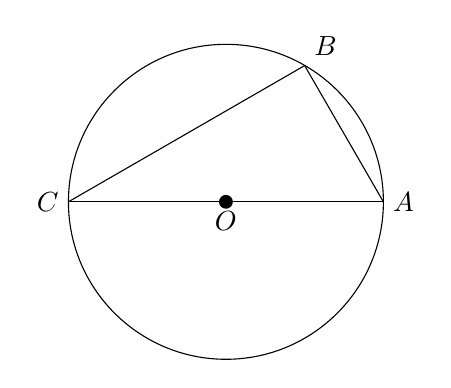
\begin{tikzpicture}
                \coordinate[label=below:$O$] (O) at (0, 0);
                \coordinate[label=right:$A$] (A) at (2, 0);
                \coordinate[label=above right:$B$] (B) at (1, 1.73);
                \coordinate[label=left:$C$] (C) at (-2, 0);

                \draw (O) circle[radius=2];
                \draw (C) -- (A);
                \draw (C) -- (B);
                \draw (B) -- (A);

                \fill (O) circle[radius=2.5pt];
            \end{tikzpicture}
        \end{center}
         The diagram above shows the cross-section of a sphere containing the centre $O$ of the sphere. The points $A$, $B$ and $C$ are on the circumference of the cross-section with the line segment $AC$ passing through $O$. It is given that $\oa{OA} = \vec a$ and $\oa{OB} = \vec b$.

        \begin{enumerate}
            \item Find $\oa{BC}$ in terms of $\vec a$ and $\vec b$.
            \item $D$ is a point on $BC$ such that $\triangle OCD$ is similar to $\triangle ACB$. Find $\oa{OD}$ in terms of $\vec a$ and $\vec b$.
        \end{enumerate}

         Point $B$ lies on the $x$-$z$ plane and has a positive $z$-component. It is also given that $\oa{OC} = \cveciii200$ and $\angle OCB = \dfrac\pi6$.

        \begin{enumerate}
            \setcounter{enumi}{2}
            \item Show that $\oa{OB} = \cveciii{-1}0{\sqrt3}$.
            \item Hence, determine whether the line passing through $O$ and $B$ and the line $\dfrac{x-2}3 = \dfrac{y}3 = z-1$ are skew.
        \end{enumerate}

    \solution
        \part
            By symmetry, we have $\oa{OC} = -\oa{OA}$. Hence,
            \begin{alignat*}{2}
                &&\oa{OC} &= -\oa{OA}\\
                \implies&&\oa{OB} + \oa{BC} &= -\oa{OA}\\
                \implies&&\oa{BC} &= -\oa{OA} - \oa{OB}\\
                && &= -\vec a - \vec b
            \end{alignat*}

            \boxt{$\oa{BC} = -\vec a - \vec b$}

        \part
            \begin{center}
                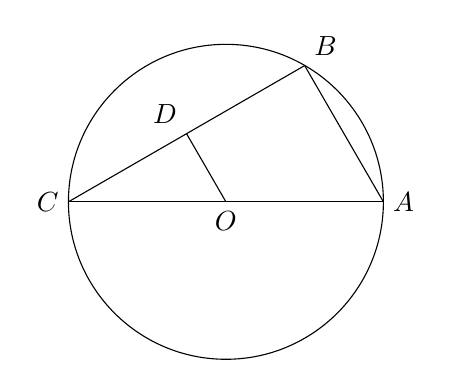
\begin{tikzpicture}
                    \coordinate[label=below:$O$] (O) at (0, 0);
                    \coordinate[label=right:$A$] (A) at (2, 0);
                    \coordinate[label=above right:$B$] (B) at (1, 1.73);
                    \coordinate[label=left:$C$] (C) at (-2, 0);
                    \coordinate[label=above left:$D$] (D) at (-0.5, 0.865);

                    \draw (O) circle[radius=2];
                    \draw (C) -- (A);
                    \draw (C) -- (B);
                    \draw (B) -- (A);
                    \draw (O) -- (D);
                \end{tikzpicture}
            \end{center}

             Since $\triangle OCD$ is similar to $\triangle ACB$, we have $\dfrac12 = \dfrac{OC}{AC} = \dfrac{OD}{AB} \implies OD = \dfrac12 AB$. Since $\oa{AB} = \vec b - \vec a$, we have
            \boxt{$\oa{OD} = \dfrac12 (\vec b - \vec a)$}

        \part
            \begin{center}
                \begin{tikzpicture}
                    \coordinate[label=below:$O$] (O) at (0, 0);
                    \coordinate[label=right:$A$] (A) at (2, 0);
                    \coordinate[label=above right:$B$] (B) at (1, 1.73);
                    \coordinate[label=left:$C$] (C) at (-2, 0);
                    \coordinate[label=below:$F$] (F) at (1, 0);

                    \draw (O) circle[radius=2];
                    \draw (C) -- (A);
                    \draw (C) -- (B);
                    \draw (B) -- (A);
                    \draw (O) -- (B);
                    \draw[dotted] (B) -- (F);

                    \draw pic [draw, angle radius=5mm, ""] {angle = O--C--B};
                    \draw pic [draw, angle radius=5mm, ""] {angle = A--O--B};

                    \draw (-1, -0.1) -- (-1, 0.1);
                    \draw (1, -0.1) -- (1, 0.1);
                    \draw[rotate=60] (1, -0.1) -- (1, 0.1);
                \end{tikzpicture}
            \end{center}

             It is given that $\angle OCB = \dfrac\pi6$. Since the angle at the centre is twice the angle at the circumference, we have $\angle AOB = 2 \angle OCB = \dfrac\pi3$. Since $OB = OA$, it must be that $\triangle OAB$ is equilateral. Let $F$ be the foot of the perpendicular from $B$ to $OA$. Note that $OB = OC = 2$. Thus, $\cos \angle AOB = \dfrac{OF}{OB} \implies OF = 1 \implies \oa{OF} = \cveciii{-1}00$. Further, note that $\sin \angle AOB = \dfrac{FB}{OB} \implies FB = \sqrt{3}$. Since $\oa{OB}$ has a positive $z$-component, we have
            \begin{align*}
                \oa{OB} &= \oa{OF} + \oa{FB}\\
                &= \cveciii{-1}00 + \cveciii00{\sqrt3}\\
                &= \cveciii{-1}0{\sqrt3}
            \end{align*}

            \boxt{$\oa{OB} = \cveciii{-1}0{\sqrt3}$}
            
        \part
            Observe that the line with Cartesian equation $\dfrac{x-2}3 = \dfrac{y}3 = z-1$ has vector equation
            \[
                l_C : \vec r = \cveciii201 + \l \cveciii331, \, \l \in \R
            \]
            Also note that the line $OB$ has equation
            \[
                l_{OB} : \vec r = \m\cveciii{-1}0{\sqrt3}, \, \m \in \R
            \]
            Consider $l_C = l_{OB}$.
            \begin{alignat*}{2}
                &&l_C &= l_{OB}\\
                \implies&&\cveciii201 + \l \cveciii331 &= \m\cveciii{-1}0{\sqrt3}\\
                \implies&&\m\cveciii{-1}0{\sqrt3} - \l \cveciii331 &= \cveciii201
            \end{alignat*}
            This gives the system
            \[
                \systeme{-\m-3\l=2,-3\l=0,\sqrt3 \m-\l=1}
            \]
            which has no solutions. Hence, the line are skew.
            
            \boxt{The lines are skew.}

    \problem{NYJC Prelim 9758/2017/02/Q1}
        The position vectors of points $A$ and $B$ with respect to the origin $O$ are $\vec a$ and $\vec b$ respectively where $\vec a$ and $\vec b$ are non-zero vectors. Point $C$ lies on $OA$ produced such that $4OA = AC$ and point $D$ lies on $OB$ produced such that $OB = BD$. The line $BC$ and $AD$ meet at the point $M$.

        \begin{enumerate}
            \item Giving a necessary condition for $\vec a$ and $\vec b$, find the position vector of $M$ in terms of $\vec a$ and $\vec b$.
            \item If $\abs{\vec a} = 1$ and $\abs{\vec b} = 2$, find the shortest distance of $M$ from the line $OC$, giving your answer in the form $k\abs{\vec a \crossp \vec b}$, where $k$ is a constant to be determined.
        \end{enumerate}

    \solution
        \part
            \boxt{$\vec a$ and $\vec b$ must be non-parallel.}

             Note that $\oa{OC} = 5\vec a$ and $\oa{OD} = 2\vec b$. Hence, $\oa{AD} = 2\vec b - \vec a$ and $\oa{BC} = 5\vec a - \vec b$. Thus, the lines $AD$ and $BC$ have vector equations
            \begin{align*}
                l_{AD} : \vec r &= \vec a + \l(2\vec b - \vec a), \, \l \in \R\\
                l_{BC} : \vec r &= \vec b + \m(5\vec a - \vec b), \, \m \in \R
            \end{align*}
            Consider $l_{AD} = l_{BC}$.
            \begin{alignat*}{2}
                &&l_{AD} &= l_{BC}\\
                \implies&&\vec a + \l(2\vec b - \vec a) &= \vec b + \m(5\vec a - \vec b)
            \end{alignat*}
            Comparing coefficients of $\vec a$ and $\vec b$, we have the system
            \[
                \systeme{1-\l=5\m,2\l=1-\m}
            \]
            which has solution $\l = \dfrac49$ and $\m = \dfrac19$. Thus,
            \begin{align*}
                \oa{OM} &= \vec b + \dfrac19 (5\vec a - \vec b)\\
                &= \dfrac59 \vec a + \dfrac89 \vec b
            \end{align*}

            \boxt{$\oa{OM} = \dfrac59 \vec a + \dfrac89 \vec b$}

        \part
            \begin{center}
                \begin{tikzpicture}
                    \coordinate[label=below:$O$] (O) at (0, 0);
                    \coordinate[label=below:$A$] (A) at (1, 0);
                    \coordinate[label=above left:$B$] (B) at (1, 2);
                    \coordinate[label=below:$C$] (C) at (5, 0);
                    \coordinate[label=above:$D$] (D) at (2, 4);
                    \coordinate[label=above right:$M$] (M) at (13/9, 16/9);
                    \coordinate[label=below:$F$] (F) at (13/9, 0);

                    \draw (O)--(C);
                    \draw (O)--(D);
                    \draw (B)--(C);
                    \draw (A)--(D);
                    \draw[dotted] (F)--(M);
                \end{tikzpicture}
            \end{center}
            
             Let $F$ be the foot of the perpendicular of $M$ to $OC$. Observe that $\oa{OM} = \dfrac59 \vec a + \dfrac89 \vec b - \vec a = -\dfrac49 \vec a + \dfrac89 \vec b$ and $\oa{AC} = 5\vec a - \vec a = 4\vec a$.
            \begin{alignat*}{2}
                &&\abs{\oa{AM} \crossp \oa{AC}} &= 2 \area \triangle AMC\\
                \implies&&\abs{\bp{-\dfrac49 \vec a + \dfrac89 \vec b} \crossp 4\vec a} &= 2 \cdot \dfrac12 \cdot FM \cdot AC\\
                \implies&&\abs{-\dfrac{16}9\vec a \crossp \vec a + 4 \cdot \dfrac89 \vec b \crossp \vec a} &= FM \cdot \abs{4 \vec a}\\
                \implies&&4 \cdot \dfrac89 \cdot \abs{\vec b \crossp \vec a} &= 4 \cdot FM\\
                \implies&&FM &= \dfrac89 \abs{\vec b \crossp \vec a}\\
                && &=  \dfrac89 \abs{\vec a \crossp \vec b}
            \end{alignat*}

            \boxt{The shortest distance of $M$ from the line $OC$ is $\dfrac89 \abs{\vec a \crossp \vec b}$ units.}

    \problem{PJC Prelim 9758/2017/02/Q1}
        Referred to the origin $O$, points $A$ and $B$ have position vectors $\vec a$ and $\vec b$ respectively. Point $P$ lies on $OA$ produced such that $OA : AP = 1 : \l$. Point $Q$ lies on $OB$, between $O$ and $B$, such that $OQ:QB = 3:1$. The mid-point of $PB$ is $M$. Show that the ratio of the area of triangle $OPM$ to the area of triangle $OQM$ is independent of $\l$.

    \solution
        \begin{center}
            \begin{tikzpicture}
                \coordinate[label=below:$O$] (O) at (0, 0);
                \coordinate[label=below:$A$] (A) at (4, 0);
                \coordinate[label=above:$B$] (B) at (2, 4);
                \coordinate[label=below:$P$] (P) at (6, 0);
                \coordinate[label=above left:$Q$] (Q) at ($(O)!0.75!(B)$);
                \coordinate[label=above right:$M$] (M) at ($(P)!0.5!(B)$);

                \draw (O)--(B);
                \draw (O)--(P);
                \draw (P)--(B);
                \draw (O)--(M);
                \draw (M)--(Q);
                
                \fill (A) circle[radius=2.5pt];

                \node at ($(O)!0.5!(M)!0.333!(P)$) {$X$};
                \node at ($(O)!0.5!(M)!0.333!(Q)$) {$Y$};
                \node at ($(B)!0.5!(M)!0.333!(Q)$) {$Z$};
            \end{tikzpicture}
        \end{center}

         Let the area of $\triangle OPM$, $\triangle OQM$ and $\triangle BQM$ be $X$, $Y$ and $Z$ respectively. Since $\triangle OPM$ and $\triangle BOM$ share the same height and $BM = MP$, we have
        \[
            X = Y + Z
        \]
        Similarly, since $\triangle OQM$ and $\triangle BQM$ share the same height and $OQ = 3QM$, we have
        \[
            Y = 3Z
        \]
        Thus, $X = Y + \dfrac13 Y$, whence $\dfrac{\area \triangle OPM}{\area \triangle OQM} = \dfrac{X}{Y} = \dfrac43$. Thus, the required ratio is independent of $\l$.

    \problem{RI Prelim 9758/2017/02/Q1}
        Referred to the origin $O$, the points $A$, $B$ and $C$ have position vectors $\vec a$, $\vec b$ and $\vec c$ respectively such that
        \begin{align*}
            \vec a &= 2\vec i + 3\vec j - \vec k\\
            \vec b &= 5\vec i - 2\vec j + 3\vec k\\
            \vec c &= 4\vec i + \vec j - 2\vec k
        \end{align*}

        \begin{enumerate}
            \item Given that $M$ is the mid-point of $AC$, use a vector product to find the exact area of triangle $ABM$.
            \item Find the position vector of the point $N$ on the line $AB$ such that $\oa{MN}$ is perpendicular to $\oa{AB}$.
        \end{enumerate}

    \solution
        We have $\vec a = \cveciii23{-1}$, $\vec b = \cveciii5{-2}3$ and $\vec c = \cveciii41{-2}$.

        \part
            By the Midpoint Theorem, $\oa{OM} = \dfrac12 (\vec a + \vec c) = \cveciii32{-3/2}$. Thus, $\oa{AM} = \cveciii1{-1}{-1/2}$. We also have $\oa{AB} = \cveciii3{-5}4$. Hence,
            \begin{align*}
                \area \triangle ABM &= \dfrac12 \abs{\oa{AM} \crossp \oa{AB}}\\
                &= \dfrac12 \abs{\cveciii1{-1}{-1/2} \crossp \cveciii3{-5}4}\\
                &= \dfrac14 \abs{\cveciii{-2}2{1} \crossp \cveciii3{-5}4}\\
                &= \dfrac12 \abs{\cveciii{13}{11}4}\\
                &= \dfrac{\sqrt{306}}4\\
                &= \dfrac{3\sqrt{34}}4
            \end{align*}

            \boxt{$\area \triangle ABM = \dfrac{3\sqrt{34}}4$ units$^2$}

        \part
            Note that the line $AB$ has vector equation
            \[
                l_{AB} : \vec r = \cveciii23{-1} + \l\cveciii3{-5}4, \, \l \in \R
            \]
            Since $\oa{MN}$ is perpendicular to $\oa{AB}$, we have
            \begin{alignat*}{2}
                &&\oa{MN} \cdot \oa{AB} &= 0\\
                \implies&&\bp{\oa{ON} - \oa{OM}} \cdot \cveciii3{-5}4 &= 0\\
                \implies&&\left[\cveciii23{-1} + \l\cveciii3{-5}4 - \cveciii32{-3/2}\right] \cdot \cveciii3{-5}4 &= 0\\
                \implies&&\left[\cveciii{-1}1{1/2} + \l\cveciii3{-5}4\right] \cdot \cveciii3{-5}4 &= 0\\
                \implies&&\cveciii{-1}1{1/2} \cdot \cveciii3{-5}4 + \l\cveciii3{-5}4 \cdot \cveciii3{-5}4 &= 0\\
                \implies&&-6 + 50\l &= 0\\
                \implies&&\l &= \dfrac3{25}
            \end{alignat*}

            Hence, $\oa{ON} = \cveciii23{-1} + \dfrac3{25}\cveciii3{-5}4 = \dfrac1{25} \cveciii{59}{60}{-13}$.

            \boxt{$\oa{ON} = \dfrac1{25} \cveciii{59}{60}{-13}$}
\end{document}